\begin{frame}{What can an audit record tell us?}
An administration audits 100 firms and finds discrepancies in 30.
\par\vspace{4mm}
\begin{center}{\Huge\color{Teal}30\%}\end{center}
\prompt{Does this mean that 30\% of all firms have a discrepancy?\\What would you need to know first?}
\source{Hypothetical example. No real tax records or estimates.}
\note{Opening discussion, 8 minutes. Ask first how the 100 firms were selected. Separate an observed discrepancy from an intentional offence. Do not introduce formulas yet.}
\end{frame}

\begin{frame}{The question determines the analysis}
\begin{tabular}{>{\raggedright\arraybackslash}p{.26\textwidth}>{\raggedright\arraybackslash}p{.63\textwidth}}
\toprule
\textbf{Question} & \textbf{What we need}\\\midrule
What happened in these records? & Description of the observed data.\\[3mm]
What happens in all firms? & Inference, with a defensible sampling or modelling framework.\\[3mm]
Which cases need review? & Prediction, evaluated on relevant new cases.\\[3mm]
Did a policy change behaviour? & A design that can support a causal comparison.\\\bottomrule
\end{tabular}\par
\end{frame}

\begin{frame}{Our route through the data analysis module}
\begin{center}\begin{tikzpicture}[every node/.style={align=center,font=\small},box/.style={draw=Teal,thick,minimum width=3.9cm,minimum height=1.1cm}]
\node[box] (a) {Describe\\measurement and distributions};
\node[box,right=7mm of a] (b) {Infer\\samples and uncertainty};
\node[box,below=8mm of a] (c) {Relate\\association and comparison};
\node[box,right=7mm of c] (d) {Learn\\prediction and structure};
\draw[-{Stealth},Teal,thick] (a)--(b);
\draw[-{Stealth},Teal,thick] (a)--(c);
\draw[-{Stealth},Teal,thick] (b)--(d);
\draw[-{Stealth},Teal,thick] (c)--(d);
\end{tikzpicture}\end{center}
At each stage: what was measured, who is represented, and what does the result justify?
\end{frame}

\begin{frame}{The first meeting}
\begin{tabular}{l>{\raggedright\arraybackslash}p{.74\textwidth}}\toprule
14:30--14:45 & Course organisation, survey and opening audit question.\\[2mm]
14:45--15:05 & A diagnostic discussion of statistical reasoning.\\[2mm]
15:05--15:30 & A shared dataset: measurement, summaries and interpretation.\\[2mm]
15:30--15:40 & Break.\\[2mm]
15:40--16:00 & Fiscal records, tax compliance and human-centred AI.\\[2mm]
16:00--16:20 & R and the two independent e-tivities.\\[2mm]
16:20--16:30 & Exit questions and preparation for 4 November.\\\bottomrule
\end{tabular}\par
\end{frame}

\begin{frame}{Our meetings in 2026}
\small
\begin{tabular}{ll>{\raggedright\arraybackslash}p{.60\textwidth}}\toprule
\textbf{Date} & \textbf{Time} & \textbf{Proposed focus}\\\midrule
14 October & 14:30--16:30 & Introduction and launch of independent activities\\
4 November & 14:30--16:30 & Debrief and introduction to inference\\
6 November & 10:30--12:30 & Bivariate analysis\\
11 November & 14:30--16:30 & R laboratory: description, inference, association\\
13 November & 10:30--12:30 & Introduction to statistical learning\\
18 November & 14:30--16:30 & Supervised learning\\
20 November & 10:30--12:30 & R laboratory: supervised learning\\
25 November & 14:30--16:30 & Unsupervised learning\\
27 November & 10:30--12:30 & R laboratory: unsupervised learning\\
2 December & 14:30--16:30 & Applications to open data\\
4 December & 10:30--12:30 & Applications and synthesis\\\bottomrule
\end{tabular}\par
\source{All meetings: room 424. Dates, times and room from the supplied tentative timetable. Topic allocation is a teaching proposal. The full course timetable also includes Chiara Francioso's meetings.}
\end{frame}

\begin{frame}{Six e-tivities across the module}
\begin{tabular}{cl>{\raggedright\arraybackslash}p{.49\textwidth}}\toprule
 & \textbf{E-tivity} & \textbf{Purpose}\\\midrule
1 & Counting and taxation & From fiscal records to compliance\\[2mm]
2 & Descriptive statistics & A shared set of prerequisites\\[2mm]
3 & Inference & Sampling variability and uncertainty\\[2mm]
4 & Bivariate analysis & Relationships between variables\\[2mm]
5 & Supervised learning & Prediction and validation\\[2mm]
6 & Unsupervised learning & Structure, distances and interpretation\\\bottomrule
\end{tabular}\par
\par\vspace{2mm}Activities 1 and 2 prepare the return to class on 4 November.\\
The remaining activities will accompany the later blocks.
\end{frame}

\begin{frame}{Before 4 November}
\begin{columns}[T]
\column{.47\textwidth}\textbf{1. Counting and taxation}\\
Allow about 60--90 minutes.\\
Explore fiscal records and Petty, compare assessments and payments, then connect the evidence to AI.\\
Bring a short reflection and one question.
\column{.47\textwidth}\textbf{2. Descriptive statistics}\\
Allow about 2--2.5 hours, in two sessions.\\
Review concepts, explore the interactive examples, and analyse the supplied data.\\
Bring a short analysis and your unresolved questions.
\end{columns}
\par\vspace{4mm}The activities provide formative feedback. Keep your exported answers for the classroom debrief.
\note{Suggested pacing: history during 15--21 October, descriptive sections during 22 October--3 November. Estimated duration depends on prior knowledge.}
\end{frame}

\begin{frame}{Course information and support}
\begin{itemize}
\item Course announcements and teaching materials: \href{https://myariel.unimi.it/course/view.php?id=3315}{ARIEL course page}.
\item Contact: \href{mailto:silvia.salini@unimi.it}{silvia.salini@unimi.it}.
\item Arrange an appointment by email.
\item Use the supplied GitHub activity files for practice and save your work locally.
\item The official course page will confirm assessment arrangements.
\end{itemize}\source{The ARIEL address is retained from the supplied introductory slides.}
\note{Check that the retained ARIEL course address refers to the current course. The old Friday office hours and the old survey link have deliberately not been treated as current. The original slides mention an oral examination and a possible project: confirm the current arrangements before announcing them.}
\end{frame}

\begin{frame}{Class survey and entry test}
\begin{columns}[c]
\column{.48\textwidth}
\textbf{Data Analysis and Tax Compliance}\\
Academic year 2026/2027\\[5mm]
Scan the QR code with your phone.\\[3mm]
Complete the class survey and entry test before our diagnostic discussion.
\column{.47\textwidth}
\centering
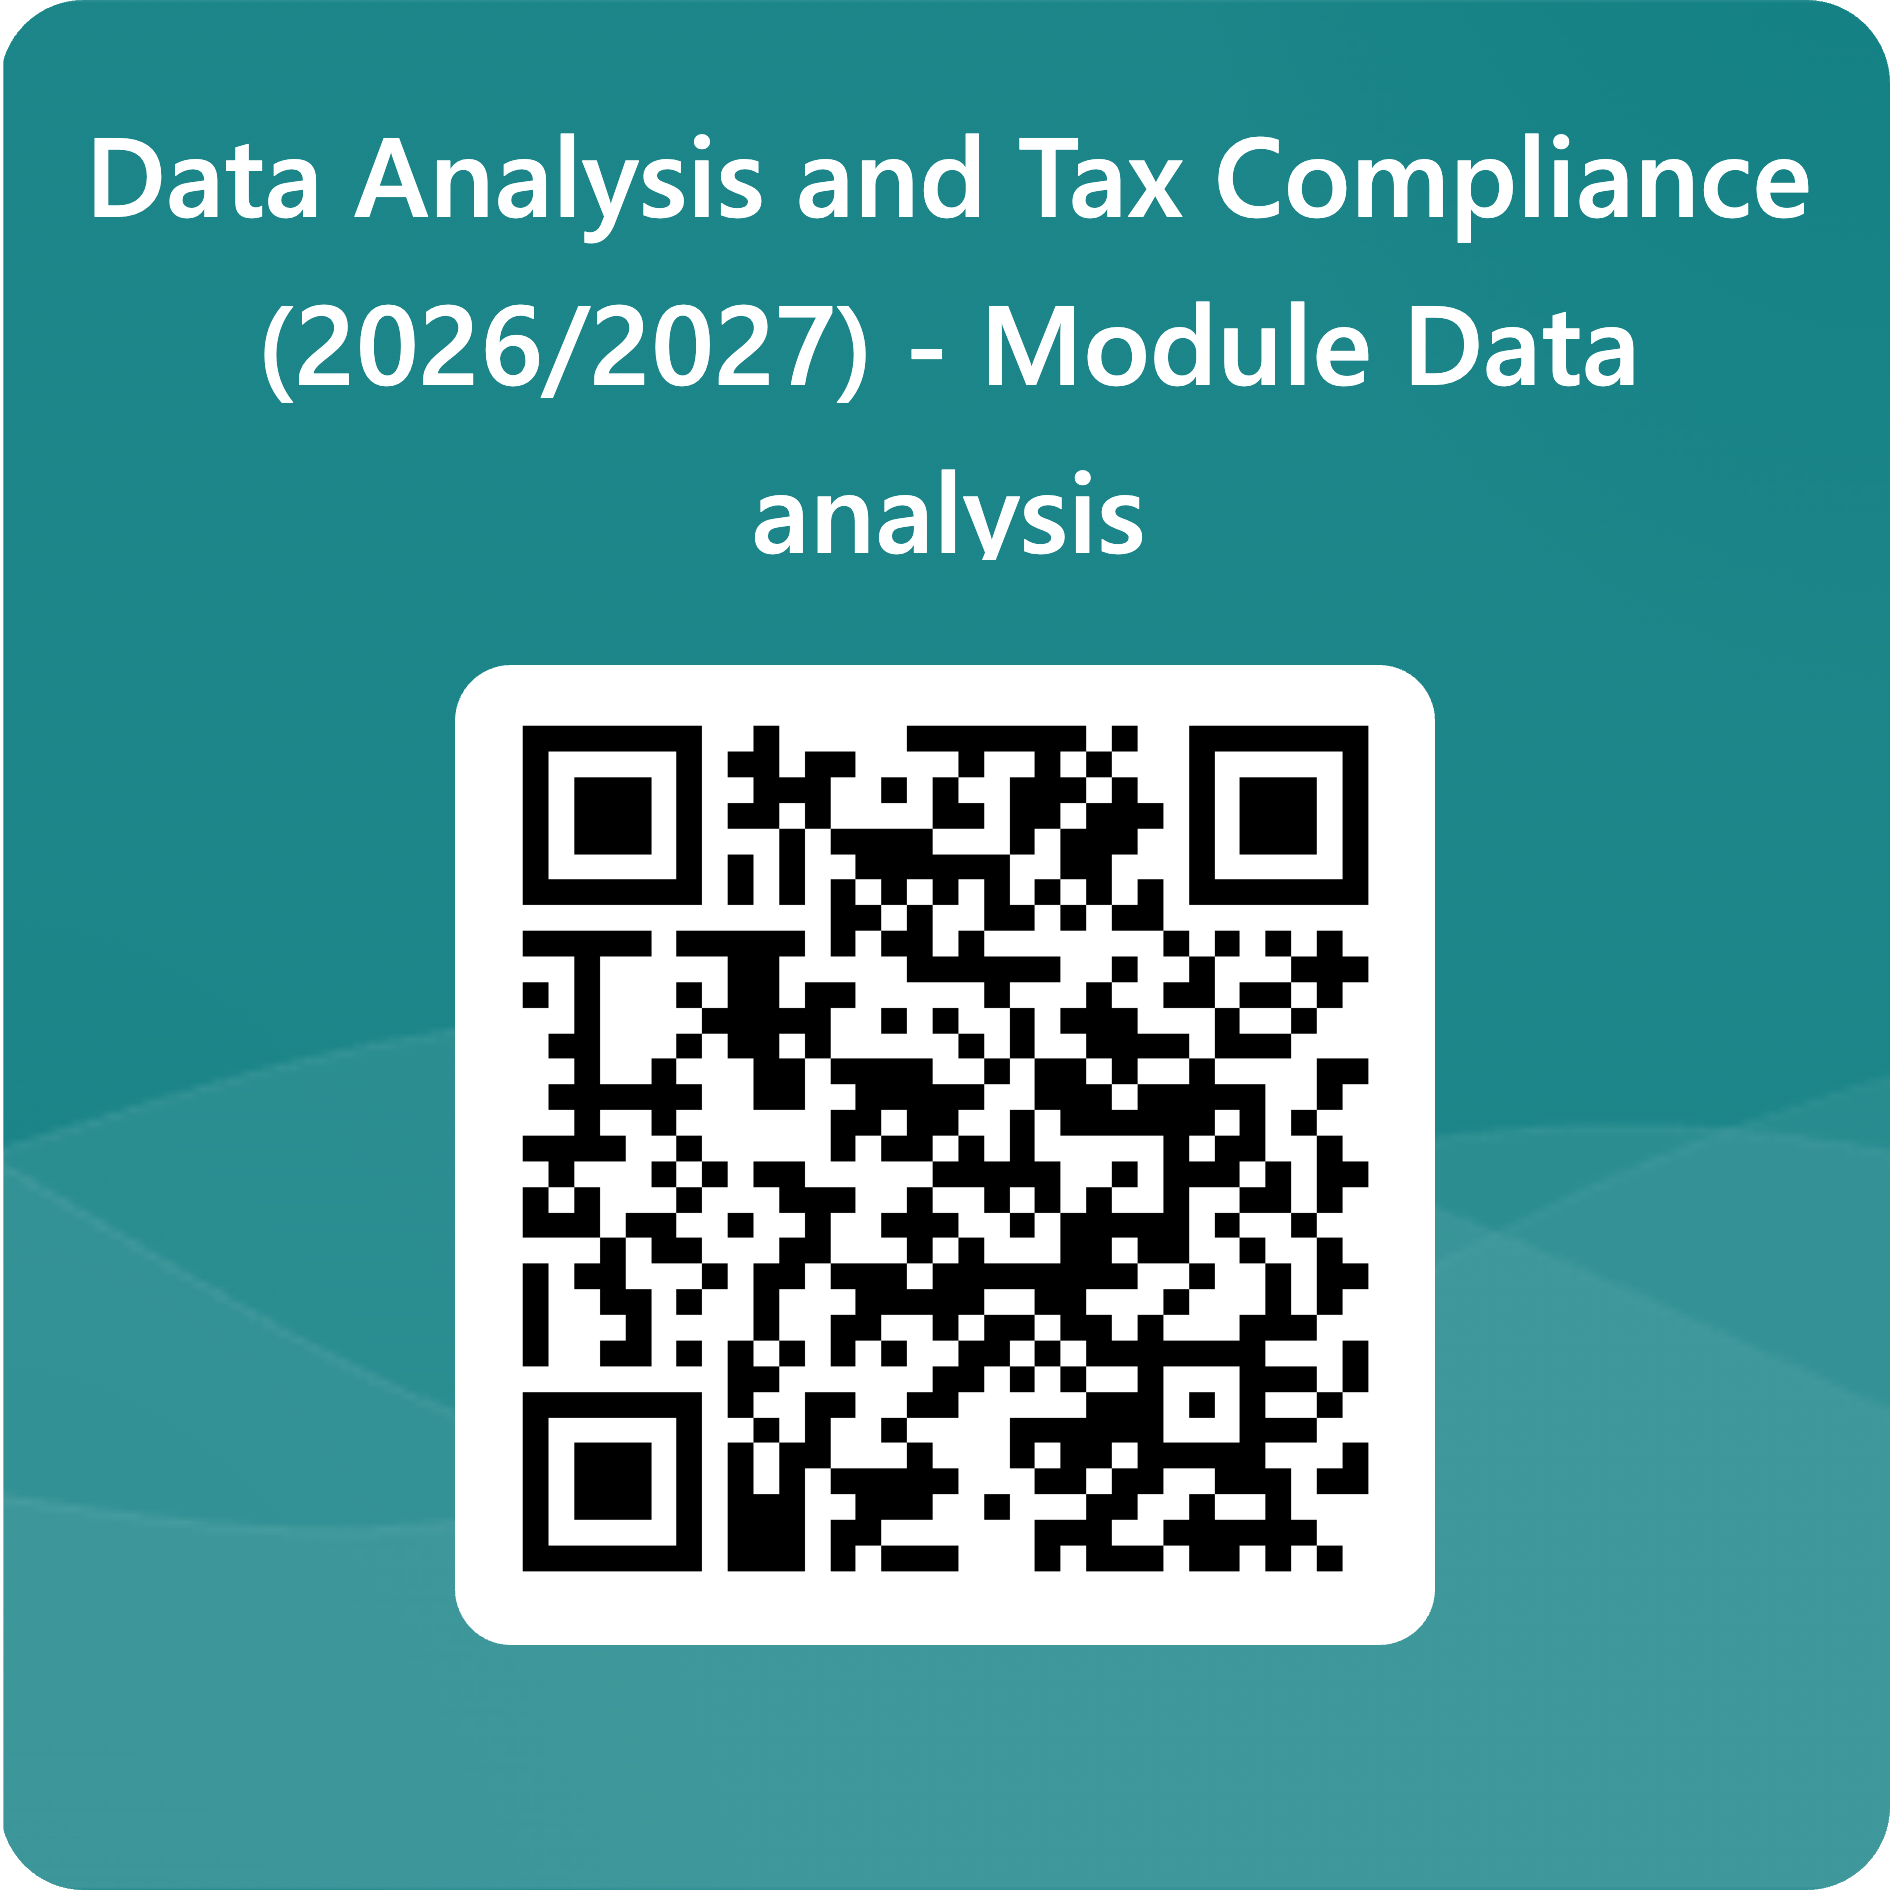
\includegraphics[width=5.2cm,trim=380bp 200bp 380bp 560bp,clip]{figures/class-survey.png}
\end{columns}
\note{Use the QR code supplied for the 2026/2027 data-analysis module. The original PNG is included unchanged in the project; the slide displays its QR region.}
\end{frame}

\begin{frame}{A diagnostic discussion}
\begin{itemize}
\item A sample contains a million records. Must it represent the population?
\item Can two datasets have the same mean and very different distributions?
\item A firm has $z=1.5$. What does this tell us?
\item An algorithm flags a case. Is this evidence of an intentional violation?
\end{itemize}\prompt{Work in pairs. Explain your reasoning before using a formula.}
\note{Allow 10 minutes in pairs and 10 minutes of discussion. Answers: no; yes; 1.5 standard deviations above the reference mean; no, a flag requires investigation. Use answers to prioritise the independent review.}
\end{frame}

\begin{frame}{Our shared dataset}
\small
\begin{tabular}{llllrr}\toprule
Firm & Sector & Channel & Audited & Turnover & Delay\\
 & & & & (thousand EUR) & (days)\\\midrule
F01 & Commerce & Paper & 0 & 18 & 0\\
F02 & Commerce & Online & 0 & 20 & 0\\
F03 & Commerce & Online & 1 & 20 & 0\\
F24 & Manufacturing & Online & 1 & 300 & missing\\\bottomrule
\end{tabular}\par
\par\vspace{3mm}\normalsize
24 fictional firms, one filing per firm for a single reference year.\\
The file also records whether an audit found a discrepancy.\\
\alert{All records are synthetic. They describe no real firms or tax system.}
\end{frame}

\begin{frame}{The unit comes before the variable}
\begin{columns}[T]\column{.46\textwidth}
\textbf{Unit of analysis}\\
Here: one firm and its filing for the reference year.\\
A table of invoices would have a different unit.
\column{.48\textwidth}\textbf{Variable}\\
Sector is categorical.\\
Turnover is quantitative.\\
Delay is a count of days.\\
The firm identifier labels the record.
\end{columns}
\prompt{If one firm generates 1,000 invoices, how could an invoice-level mean differ from a firm-level mean?}
\end{frame}

\begin{frame}{Missing is different from zero}
\begin{columns}[T]\column{.48\textwidth}
\textbf{Zero delay}\\
The filing is on time under the definition used in this teaching dataset.
\par\vspace{3mm} \textbf{Missing delay}\\
The delay is unrecorded. We do not know whether it is zero.
\column{.46\textwidth}\textbf{No audit}\\
The discrepancy outcome is unobserved.\\
It cannot be recoded as ``no discrepancy''.
\end{columns}
\prompt{What denominator should appear in a reported percentage?}
\end{frame}

\begin{frame}{A graph makes different features visible}
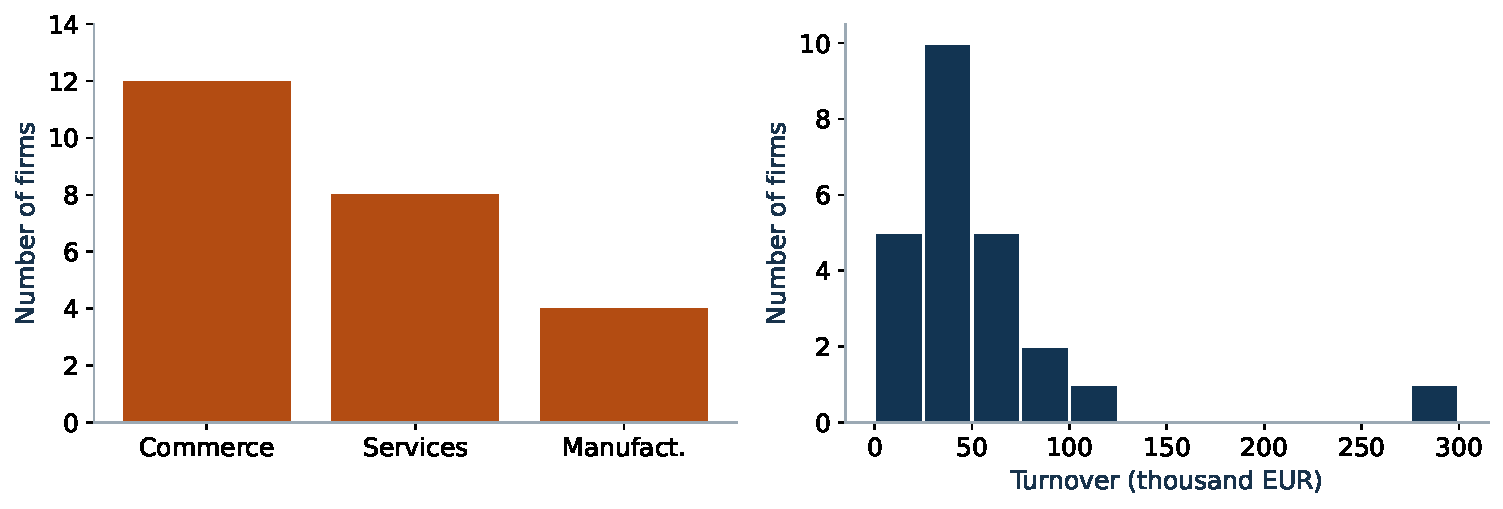
\includegraphics[width=.93\textwidth,height=4.5cm,keepaspectratio]{figures/distributions.pdf}
\prompt{Which graph answers a question about categories? Which reveals the long right tail?}
\end{frame}

\begin{frame}{The typical firm depends on the question}
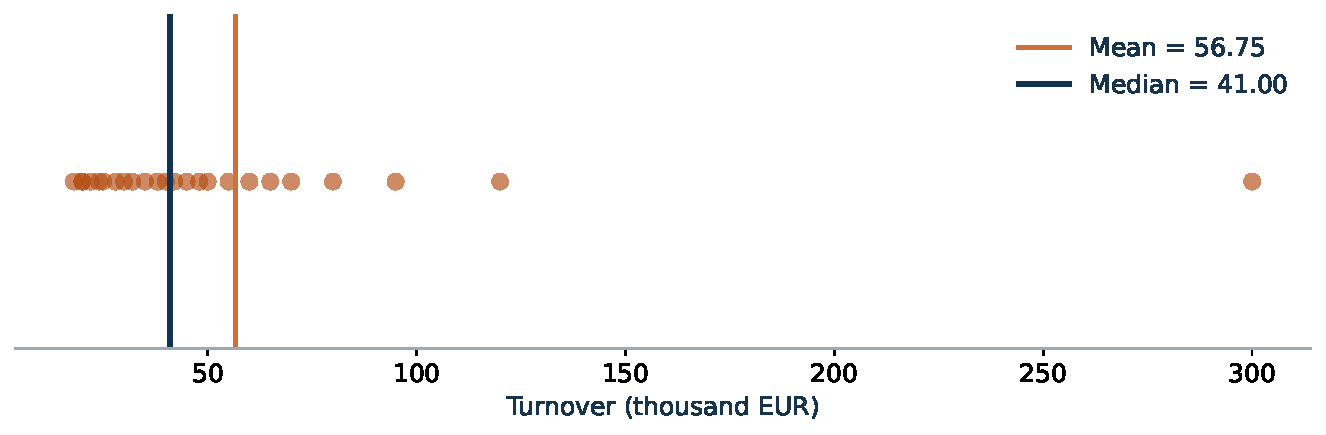
\includegraphics[width=\textwidth]{figures/centre.pdf}
\textbf{Mean:} the turnover per firm if the total were redistributed equally.\\
\textbf{Median:} the middle of the ordered observations.\\
Both are meaningful. They answer different descriptive questions.
\end{frame}

\begin{frame}{The mean leaves out the spread}
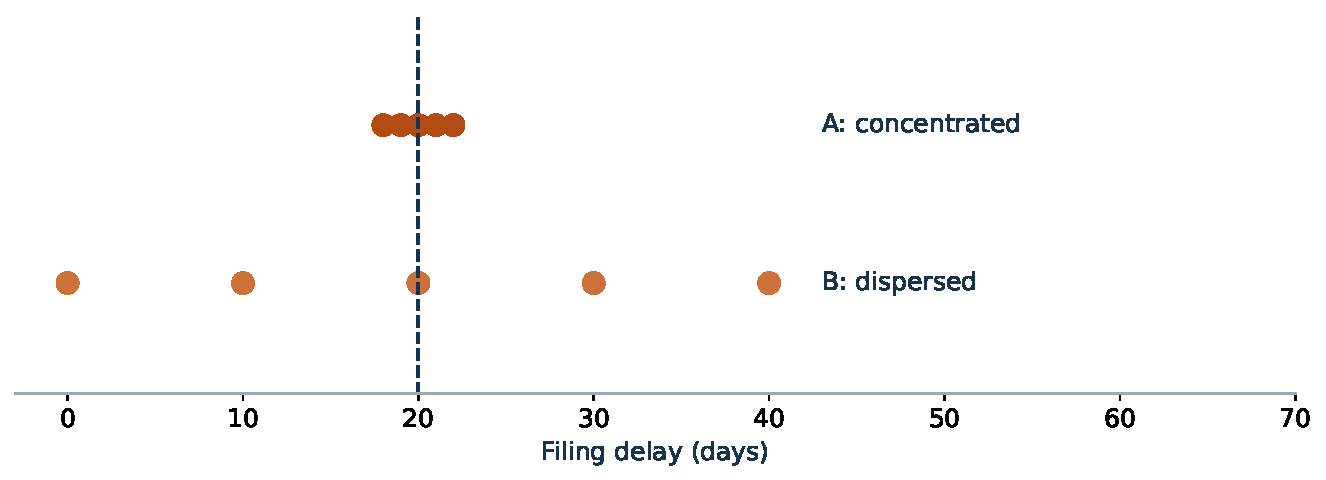
\includegraphics[width=\textwidth]{figures/spread.pdf}
Both groups have mean 20 days. Group B varies much more.\\
A summary of the centre should be accompanied by a description of spread.
\end{frame}

\begin{frame}{Audit outcomes depend on selection}
In the teaching data, 10 firms were audited and 6 had a recorded discrepancy.
\begin{center}{\Large $6/10=60\%$}\end{center}
This describes the audited firms. The other 14 outcomes are unobserved.
\prompt{If audits targeted suspected cases, why might this percentage differ from the percentage among all firms?}
\source{Synthetic example. A discrepancy is not a legal determination or a measure of intention.}
\end{frame}

\begin{frame}{Statistical reasoning begins with a question}
\begin{enumerate}
\item State a question that can be investigated.
\item Define what the observations and measurements represent.
\item Examine the data and the process that generated them.
\item Choose an analysis appropriate to the question.
\item Interpret the result, its uncertainty and its limits.
\end{enumerate}
\prompt{Where could an error enter before any calculation is made?}
\end{frame}

\begin{frame}{Fiscal administration: one root of statistical records}
\textbf{Who is liable? What resources are recorded? What is owed?}
\par\vspace{3mm}
Roman censuses registered citizens and property for public administration, including taxation and civic obligations.
\par\vspace{3mm}
Such records made people and resources administratively visible.\\
Their coverage followed the institutions and purposes that created them.
\prompt{Would a headcount be enough to allocate a tax burden?}
\source{ONS, \href{https://www.ons.gov.uk/census/2011census/howourcensusworks/aboutcensuses/censushistory/censustakingintheancientworld}{Census-taking in the ancient world}. Administrative registers are not yet modern statistical inference.}
\end{frame}

\begin{frame}{1086: land, resources and the Domesday survey}
\begin{itemize}
\item William I's survey recorded landholding, resources and valuations in England.
\item Property information helped the Crown understand its fiscal resources.
\item It was \textbf{not a census of every person}.
\end{itemize}
\prompt{What does a property register reveal that a headcount does not? Who or what could remain outside its scope?}
\source{The National Archives, \href{https://www.nationalarchives.gov.uk/help-with-your-research/research-guides/domesday-book/}{Domesday Book research guide}.}
\end{frame}

\begin{frame}{1662: Petty on counting and tax burdens}
\textit{A Treatise of Taxes and Contributions}, chapter VII.
\begin{itemize}
\item A headcount can make a fixed charge easy to calculate.
\item A title or rank need not measure a person's resources.
\item Charging the same amount can impose unequal burdens.
\end{itemize}
\prompt{Which part is a measurement problem? Which part requires a principle for allocating the burden?}
\source{William Petty (1662), \href{https://www.gutenberg.org/cache/epub/61588/pg61588-images.html}{A Treatise of Taxes and Contributions}, chapter VII, paragraphs 2--6. Paraphrase for discussion.}
\end{frame}

\begin{frame}{Same headcount, different possible assessments}
\small
\begin{tabular}{lrrrr}\toprule
 & Households & Property value & By headcount & By property\\\midrule
District A & 100 & 800 & 100 & 160\\
District B & 100 & 200 & 100 & 40\\\midrule
Total & 200 & 1,000 & 200 & 200\\\bottomrule
\end{tabular}\par\vspace{3mm}\normalsize
Both rules raise 200 monetary units.\\
Equal household charges imply 12.5\% and 50\% of property value.\\
Property-proportional charges imply 20\% in each district.
\prompt{Data describe the consequences. What principle would justify the chosen rule?}
\source{Invented teaching example, not a reconstruction of historical taxation or current law. Property is the illustrative base.}
\end{frame}

\begin{frame}{Assessment and compliance ask different questions}
\small
\begin{columns}[T]
\column{.47\textwidth}\textbf{Assessment}\\
Apply a rule to determine what is owed.\\[2mm]
With the property rule: A owes 160; B owes 40.
\column{.47\textwidth}\textbf{Payment}\\
Compare matched payments with assessed amounts.\\[2mm]
A pays 120: $75\%$.\\
B pays 36: $90\%$.
\end{columns}
\par\vspace{3mm}
A pays more units; B pays a higher fraction.\\
Neither ratio reveals unregistered taxpayers or unreported income.
\prompt{What must be defined before calling an indicator a measure of compliance?}
\source{Synthetic example. Same obligation, period and reference date. We use modern concepts to interpret history, not to equate different historical institutions.}
\end{frame}

\begin{frame}{Statistics also developed beyond the treasury}
\textbf{1662: John Graunt and mortality}\\
Observations on the Bills of Mortality connect recorded deaths and the study of population.
\par\vspace{4mm}
\textbf{1826: Melchiorre Gioia and statistical knowledge}\\
\textit{Filosofia della statistica}: a bridge to the wider question of how observations about society inform public decisions.
\par\vspace{4mm}
Fiscal administration is one historical thread. Demography, probability and scientific inquiry also shaped modern statistics.
\source{\href{https://wellcomecollection.org/works/ear22f7e}{Graunt (1662), Wellcome Collection}; \href{https://search.worldcat.org/title/Filosofia-della-statistica/oclc/7022381}{Gioia/Gioja (1826), bibliographic record}. Further reading in E-tivity 1.}
\end{frame}

\begin{frame}{From fiscal registers to an audit-risk model}
\begin{tabular}{>{\raggedright\arraybackslash}p{.43\textwidth}>{\raggedright\arraybackslash}p{.46\textwidth}}\toprule
\textbf{Question about a register} & \textbf{Question about training data}\\\midrule
Who and what were recorded? & Which taxpayers and outcomes are represented?\\[3mm]
Why was the information collected? & How did past audit choices shape the labels?\\[3mm]
Which decisions did it support? & What can the prediction justify today?\\\bottomrule
\end{tabular}\par
\prompt{An unobserved audit outcome is not evidence of compliance. A risk score is not a legal finding.}
\source{Course synthesis: a contemporary application of the historical questions, not a claim that historical authors anticipated machine learning.}
\end{frame}


\begin{frame}{From a predicted risk to a human decision}
A model assigns a high risk score to a filing.
\par\vspace{3mm}
\begin{tabular}{>{\raggedright\arraybackslash}p{.42\textwidth}>{\raggedright\arraybackslash}p{.48\textwidth}}\toprule
\textbf{Statistical question} & \textbf{Consequence for the decision}\\\midrule
Who supplied the training data? & Some firms may be poorly represented.\\[2mm]
What does the outcome measure? & Past audit findings may reflect audit selection.\\[2mm]
Which errors occur? & False alarms and missed cases have different costs.\\[2mm]
How well does it work on new data? & Performance can change across groups and settings.\\\bottomrule
\end{tabular}\par
\end{frame}

\begin{frame}{R makes an analysis reproducible}
\begin{itemize}
\item R is the statistical computing language used in the module.
\item RStudio provides an interface for writing and running R code.
\item A script records each step, from reading a file to creating a graph.
\item Save the data, code and definitions needed to understand your results.
\end{itemize}\source{\href{https://www.r-project.org/}{R Project}\quad\href{https://posit.co/download/rstudio-desktop/}{RStudio}\quad\href{https://posit.cloud/}{Posit Cloud}}
\end{frame}

\begin{frame}[fragile]{A short, reproducible analysis}
\begin{lstlisting}[language=R]
d <- read.csv("filings_synthetic.csv")
table(d$sector)
mean(d$turnover_kEUR)
median(d$turnover_kEUR)
sd(d$turnover_kEUR)
sum(is.na(d$filing_delay_days))
\end{lstlisting}
\par\vspace{3mm}
For each output: name the variable, its unit, and the observations used.\\
The e-tivity includes a complete script and an explanation of its results.
\end{frame}
\begin{frame}{E-tivity 1: history and a contemporary problem}
\textbf{First:} complete \href{https://silviasaliniunimi.github.io/statistics-iple/01-Statistics-and-Knowledge.html}{Statistics as a Tool for Knowledge} and its self-check.
\par\vspace{2mm}
\textbf{Then:} an administration wants to use historical audits to predict future discrepancies.
\begin{enumerate}
\item Select one idea from the historical pathway.
\item Explain how it changes your approach to this problem.
\item Identify information you would request before using the model.
\end{enumerate}
Write 250--350 words. Refer to the resource you used.
\note{The HCAI activity page links to the original resource and provides a response box and export. The existing IPLE exam practice is optional, not an HCAI assessment rule.}
\end{frame}

\begin{frame}{E-tivity 2: a full descriptive review}
\begin{itemize}
\item Measurement, variable types, frequencies and missing values.
\item Graphs, centre, quantiles and the effect of extreme observations.
\item Dispersion, categorical heterogeneity and standardisation.
\item A short analysis of the 24 synthetic firms, with documented choices.
\end{itemize}\par\vspace{2mm}\textbf{Bring back:} your answers, a short report, and two questions you would like to discuss.
\end{frame}

\begin{frame}{What you should be able to do on 4 November}
\begin{itemize}
\item Describe a dataset without confusing the unit, the variable and the population.
\item Choose and interpret summaries suited to the data and the question.
\item Explain how missingness, selection and extreme values affect an analysis.
\item Distinguish a description of observed cases from a claim about a population.
\end{itemize}\prompt{Exit ticket: one concept you can explain, one choice you would check, and one question for November.}
\end{frame}

\begin{frame}{Reading and resources}
\textbf{For descriptive statistics and inference}\\
Agresti, Franklin and Klingenberg, \emph{Statistics: The Art and Science of Learning from Data}, Pearson.
\par\vspace{3mm}
\textbf{For statistical learning}\\
James, Witten, Hastie and Tibshirani, \emph{An Introduction to Statistical Learning}.\\
\href{https://www.statlearning.com/}{statlearning.com}
\par\vspace{3mm}
\textbf{For independent work}\\
The two HCAI e-tivity pages, the synthetic dataset, the R script, and the companion Beamer review.
\end{frame}

